\chapter{Task 2 - Aggregative Optimization for Multi-Robot Systems}
\label{ch:aggregative}
\section{Distributed Aggregative Optimization}
\label{sec:dist_aggr}

In this chapter, we address a coordination problem in which the goal is no longer to achieve uniform consensus, but rather to enable the emergence of a collective behavior that minimizes a global cost function. Unlike classical consensus schemes, where all agents asymptotically agree on a common state, here each agent evolves toward individual states that, together, optimize an objective function defined over the entire network. \\
A common and effective approach to this class of problems is provided by aggregative optimization, where each agent minimizes a local objective function that depends both on its own decision variable and on an aggregate quantity (typically the average) of all agents' decisions. The structure of the aggregate term allows for the development of scalable, decentralized, and privacy-preserving algorithms, often built on average-tracking dynamics or modified consensus schemes.

\medskip

\noindent This framework is particularly suitable for cooperative robotics applications. For instance, consider \( N \) robots in the plane, each optimizing its position \( z_i \in \mathbb{R}^d \), for \( i = 1, \ldots, N \), to perform multi-robot surveillance tasks. \\
Let \( r_0 \in \mathbb{R}^d \) denote a global target to protect, and \( r_i \in \mathbb{R}^d \) represent an intruder associated with robot \( i \). Define the barycenter of the robots as
\[
\sigma(z) = \frac{1}{N} \sum_{i=1}^N z_i,
\]
and let \( \gamma_i > 0 \) be a tradeoff parameter that assigns different weights to components of each robot's cost function. \\
Each robot aims to achieve two goals simultaneously: remain close to the global target \( r_0 \), and  stay close to its associated intruder \( r_i \). A simple way to express this is by considering the squared Euclidean distances between each robot and its intruder, and between the barycenter of all robots and the global target. \\
Accordingly, we define the local cost function for robot \( i \) as
\[
\ell_i(z_i, \sigma(z)) = \gamma_i \| z_i - r_i \|^2 + \| \sigma(z) - r_0 \|^2,
\]
where the first term corresponds to a private objective of staying close to the intruder (private opponent), and the second term captures a global objective of maintaining proximity to the overall target. \\
In this context, the vector \( z \in \mathbb{R}^{dN} \), formed by stacking the positions \( z_1, \ldots, z_N \), plays a different role compared to the Gradient Tracking algorithm. Here, \( z \) represents the collective positions of all robots, which collaboratively seek to minimize the total cost function by converging to an optimal configuration.

\begin{figure}[h!]
    \centering
    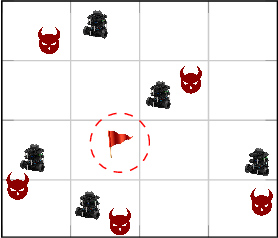
\includegraphics[width=0.35\linewidth]{figs/aggregative_optimization.png}
    \caption{Multi- robot surveillance scenario - Robot icons denote agents, devil icons denote intruders, while the flag is the target to be protected. \cite{Carnevale2021DistributedOA}}
\end{figure}

\noindent Consider aggregative optimization problems formulated as
\begin{align*}
    \min_{z_1, \dots, z_N} \quad & \sum_{i=1}^N \ell_i(z_i, \sigma(z))
\end{align*}
where the aggregative variable \(\sigma(z)\) is defined as
\[
    \sigma(z) = \frac{1}{N} \sum_{i=1}^N \phi_i(z_i)
\]
where \( z = (z_1, \ldots, z_N) \), with each \( z_i \in \mathbb{R}^{n_i} \), for all \( i = 1, \ldots, N \), and \( \ell_i : \mathbb{R}^{n_i} \times \mathbb{R}^d \rightarrow \mathbb{R} \) and \( \phi_i : \mathbb{R}^{n_i} \rightarrow \mathbb{R}^d \), for all \( i = 1, \ldots, N \).
As introduced in the previous example, the problem can be described with $\phi_i(z_i)=z_i$ representing the equally weighted barycenter.
\noindent In general, the aggregative function \(\sigma(z)\) does not have to be the barycenter specifically; rather, it must have the average form $\sigma(z) = \frac{1}{N} \sum_{i=1}^N \phi_i(z_i)$.

This form ensures that each agent contributes equally to the aggregate, enabling distributed computation and preserving symmetry among agents. The barycenter is commonly used because it offers a simple, intuitive, and fair representation of the collective influence, while maintaining the problem's traceability.

\medskip
\noindent For completeness, we present both the Centralized and Distributed Aggregative Optimization frameworks, and their comparison will be further detailed in the implementation section. \\


\paragraph{Centralized setting.}
In the centralized setting, a central coordinator has access to all agents' information and solves the global aggregative optimization problem collectively. \\  
Consider the decision variables \( z_i \in \mathbb{R}^{n_i} \) for \( i = 1, \ldots, N \). The centralized gradient descent method at iteration \( k \) updates each \( z_i \) as
\[
z_i^{k+1} = z_i^k - \alpha \left[ \nabla_{z_i} \sum_{j=1}^N \ell_j(z_j, \sigma(z_1, \ldots, z_N)) \right] \Bigg|_{z_1 = z_1^k,\, \dots,\, z_N = z_N^k}
\]
where \(\alpha > 0\) is the step size, and the notation \(\nabla_{z_i} \ell_j(\cdot)\) denotes the gradient of \(\ell_j\) with respect to the variable \(z_i\). \\
To explicitly compute the gradient, we apply the chain rule to the composite function \(\ell_j(z_j, \sigma(z))\).
The gradient at iteration \(k\) becomes
\begin{center}
    $[\nabla_{z_i} \sum_{j=1}^{N} \ell_j(z_j, \sigma(z_1, \dots, z_N))] \Bigg|_{z_1 = z_1^k,\, \dots,\, z_N = z_N^k} \in \mathbb{R}^{n_i}$ \\
    $= \nabla_1 \ell_i(z_i, \sigma) \Bigg|_{z_i = z_i^k, \sigma = \frac{1}{N}\sum_{j=1}^N \phi_j(z_j^k)} + \frac{1}{N}\nabla \phi_i(z_i) \Bigg|_{z_i = z_i^k} \cdot \sum_{j=1}^N \nabla_2 \ell_j(z_j, \sigma) \Bigg|_{z_j = z_j^k, \sigma = \frac{1}{N}\sum_{j=1}^N \phi_j(z_j^k)}$
\end{center}
where \(\nabla_1 \ell_i\) is the gradient of \(\ell_i\) with respect to its first argument \(z_i\), and \(\nabla_2 \ell_j\) is the gradient with respect to the second argument \(\sigma\). \\
From this formulation, it is evident that some terms, such as \(\nabla_1 \ell_i(z_i^k, \sigma^k)\) and \(\nabla \phi_i(z_i^k)\), can be computed locally by each agent. However, the aggregative variable \(\sigma^k\) and the summation \(\sum_{j=1}^N \nabla_2 \ell_j(z_j^k, \sigma^k)\) require global knowledge, which motivates the need for approximation techniques in distributed implementations. \\
Thus, the centralized update rule can be written as
\[
z_i^{k+1} = z_i^k - \alpha \left( \nabla_1 \ell_i(z_i^k, \sigma^k) + \frac{1}{N} \nabla \phi_i(z_i^k) \sum_{j=1}^N \nabla_2 \ell_j(z_j^k, \sigma^k) \right).
\]
Let us now derive the distributed version of this algorithm. \\

\paragraph{Distributed setting.}
In a distributed setting, each agent \(i\) has access only to its local functions \(\ell_i\) and \(\phi_i\), and maintains an estimate \(z_i^k\) of its optimal decision variable \(z_i^*\).  \\
A key challenge in this context is that the gradient computation required for the update cannot be performed locally by a single agent, as it depends on global quantities that aggregate information from all agents. \\ Specifically, the quantities 
\[
\sigma = \frac{1}{N} \sum_{j=1}^N \phi_j(z_j^k) \quad \text{and} \quad \frac{1}{N}\sum_{j=1}^N \nabla_2 \ell_j(z_j^k, \sigma)
\]
are global and thus unknown to individual agents. \\
To overcome this, each agent maintains local estimates \(s_i^k\) and \(v_i^k\) that serve as proxies for these global quantities, respectively. These proxies are dynamically updated through local communication with neighboring agents to track the true global values over time. This approach draws inspiration from the gradient tracking technique, exploiting the fact that both \(\sigma\) and the sum of gradients can be interpreted as averages, which can be tracked using dynamic consensus algorithms. \\
The distributed algorithm proceeds as follows: agent \(i\) updates its local variables according to:
\begin{align*}
z_i^{k+1} &= z_i^k - \alpha \left( \nabla_1 \ell_i(z_i^k, s_i^k) + \nabla \phi_i(z_i^k) v_i^k \right), & z_i^0 &\in \mathbb{R}^{n_i} \\
s_i^{k+1} &= \sum_{j \in \mathcal{N}_i} a_{ij} s_j^k + \phi_i(z_i^{k+1}) - \phi_i(z_i^k), & s_i^0 &= \phi_i(z_i^0) \\
v_i^{k+1} &= \sum_{j \in \mathcal{N}_i} a_{ij} v_j^k + \nabla_2 \ell_i(z_i^{k+1}, s_i^{k+1}) - \nabla_2 \ell_i(z_i^k, s_i^k), & v_i^0 &= \nabla_2 \ell_i(z_i^0, s_i^0)
\end{align*}
where the weight coefficients \(a_{ij}\) correspond to a consensus matrix consistent with the communication graph \(\mathcal{N}_i\) of agent \(i\). \\
The proxies \(s_i^k\) and \(v_i^k\) thus perform a dynamic consensus to track the evolving aggregate quantities \(\sigma\) and \(\frac{1}{N}\sum_j \nabla_2 \ell_j\), allowing each agent to approximate the global gradient information necessary for convergence while relying only on local information and neighbor communication. \\
A key aspect of this distributed algorithm is the separation of time scales between the consensus variables \((s_i^k, v_i^k)\) and the decision variables \(z_i^k\). Specifically, the consensus dynamics evolve on a fast time scale, while the updates of the decision variables happen on a slow time scale regulated by the step size \(\alpha > 0\).

\begin{center}
\begin{tikzpicture}[
    node distance=1.4cm and 2.5cm,
    every node/.style={align=center},
    ->, >=Stealth
]

% Blocchi con etichette
\node[draw, minimum width=5.2cm, minimum height=1.5cm] (slow) 
    {$z_i^{k+1} = z_i^k - \alpha(\ldots)$};
\node[above=0.05cm of slow] {\small\textbf{slow system}};

\node[below=1.4cm of slow, draw, minimum width=5.2cm, minimum height=1.8cm] (fast) 
    {$s_i^{k+1} = \sum a_{ij} s_j^k + \ldots$\\
     $v_i^{k+1} = \ldots$};
\node[above=0.05cm of fast] {\small\textbf{fast system}};

% Frecce
\draw[->] (fast.west) -- ++(-1.5,0) |- (slow.west); % loop a sinistra
\draw[->] (slow.east) -- ++(1.5,0) |- (fast.east); % freccia a destra verso il basso

\end{tikzpicture}
\end{center}

\noindent The consensus updates, involving weighted averages of neighbors' estimates combined with correction terms, enable the proxies to rapidly track the true aggregate quantities \(\sigma(z^k)\) and \( \frac{1}{N}\sum_j \nabla_2 \ell_j(z_j^k, \sigma(z^k))\). Since these updates do not depend on the step size \(\alpha\), they can converge much faster than the decision variables \(z_i^k\), which are updated incrementally with step size \(\alpha\). \\
The step size \(\alpha\) controls how quickly each agent adjusts its decision variable \(z_i^k\) in response to gradient information. A smaller \(\alpha\) causes the decision variables to evolve more slowly, effectively allowing the consensus variables \(s_i^k\) and \(v_i^k\) to track the aggregate quantities accurately before significant changes in \(z_i^k\) occur. This slow evolution relative to the fast consensus ensures that gradient computations use up-to-date global information, preventing divergence due to stale or inaccurate estimates. \\
Mathematically, this can be viewed as a two-time-scale dynamical system, where the fast dynamics correspond to consensus on \(s_i^k\) and \(v_i^k\), and the slow dynamics correspond to gradient descent steps on \(z_i^k\). Under suitable assumptions on the communication graph and smoothness and convexity properties of the cost functions, this separation enables the distributed algorithm to closely approximate the centralized gradient descent, guaranteeing convergence to the global optimum at a linear rate for sufficiently small \(\alpha\). \cite{carnevale2025unifyingtheoryframeworkdistributed}

\paragraph{Theorem: Convergence of the Algorithm} 
\label{th:aggregative}
Let's us consider a communication graph \(G\) that is strongly connected and aperiodic, with an associated consensus matrix \(A\) that is doubly stochastic. Suppose the function \(\sum_{i=1}^N \ell_i(\cdot, \sigma(\cdot))\) is strongly convex, each \(\phi_i(\cdot)\) is differentiable and Lipschitz continuous, and the gradients \(\nabla_1 \ell_i(\cdot, \cdot)\), \(\nabla_2 \ell_i(\cdot, \cdot)\), and \(\nabla \phi_i(\cdot) \nabla_2 \ell_i(\cdot, \cdot)\) are Lipschitz continuous. Under these conditions, there exists a step size \(\alpha^* > 0\) such that for all \(\alpha \in (0, \alpha^*)\), the sequences of local solution estimates \(\{ z_1^k, \ldots, z_N^k \}_{k \in \mathbb{N}}\) generated by the Distributed Aggregative Tracking algorithm satisfy
\[
\lim_{k \to \infty} \| z_i^k - z_i^\star \| = 0,
\]
at a linear rate for all agents \(i = 1, \ldots, N\).

\section{Implementation of a Distributed Aggregative Optimization Algorithm}

Consider a team of \(N\) mobile robots operating in a two-dimensional environment, so that each robot's position lies in \(\mathbb{R}^d\), with $d=2$. Let \(z_i^k \in \mathbb{R}^d\) denote the position of robot \(i\) at iteration \(k \in \mathbb{N}\), and let \(z^k \in \mathbb{R}^{dN}\) be the stacked vector containing the positions of all robots at time \(k\). \\
The objective is to design a distributed control algorithm that enables each robot to move towards a designated private target, while maintaining cohesion within the team due to communication constraints. It is possible to see an illustrative example of this setup in Figure~\ref{fig:aggregative_opt_scenario}.

\begin{figure}[h!]
    \centering
    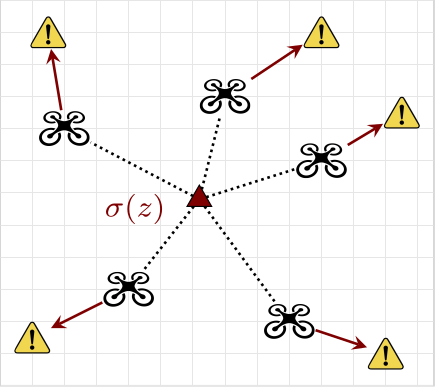
\includegraphics[width=0.3\linewidth]{figs/aggregative_opt_scenario.png}
    \caption{Example of the aggregative optimization scenario. Each robot aims to reach a private target while keeping the formation cohesive.}
    \label{fig:aggregative_opt_scenario}
\end{figure}

\noindent This scenario naturally fits within the framework of aggregative optimization, as it shares key features with the multi-robot surveillance problem introduced earlier. In this context, we define the global aggregative quantity \(\sigma(z)\) as the barycenter of the entire team, i.e.,
\[
\sigma(z) = \frac{1}{N} \sum_{j=1}^N \phi_j(z_j), \quad \text{with } \phi_j(z_j) = z_j, \ \forall j = 1, \dots, N.
\]

\paragraph{Cost function definition.} To solve this problem, the first step is to define a local cost function that captures the dual objective of staying close to the assigned target, while preserving the spatial coherence of the team.
By drawing a parallel with the multi-robot surveillance scenario introduced earlier, we can interpret each robot's private target as analogous to the intruder assigned to that robot, while the tendency to aggregate toward the barycenter reflects the need to maintain coverage or provide collective protection around a specific area, similar to the global protection objective in the surveillance setting. \\
As a first, simplified implementation, we model the local cost function as a weighted combination of two terms:
\begin{itemize}
    \item the squared Euclidean distance between the robot and its private target, encouraging convergence toward the target,
    \item the squared Euclidean distance between the robot and the team's barycenter, promoting group cohesion.
\end{itemize}

\noindent Let \(r_i \in \mathbb{R}^d\) denote the position of the target associated with robot \(i\), and let \(\gamma_i, \overline{\gamma_i} > 0\) be weights that balance the trade-off between tracking the private target and maintaining cohesion within the group. The resulting local cost function for agent \(i\) is given by:
\[
\ell_i(z_i, \sigma(z)) = \gamma_i \| z_i - r_i \|^2 + \overline{\gamma_i} \| z_i - \sigma(z) \|^2.
\] \\
In Section~\ref{sec:collision_avoidance}, we will present an enhanced version of the algorithm that incorporates collision avoidance capabilities. Specifically, we introduce a low-level safety controller that modifies the planned trajectories to ensure inter-robot collision avoidance, while the high-level distributed aggregative optimization framework governs the global coordination behavior.

\medskip

\paragraph{Centralized setting.} Following the theoretical framework, we first decided to implement the centralized algorithm before moving on to the distributed one. As introduced in the previous section, the centralized update rule is given by
\begin{align*}
z_i^{k+1} &= z_i^k - \alpha \left[ \nabla_{z_i} \sum_{j=1}^N \ell_j(z_j, \sigma(z_1, \ldots, z_N)) \right] \Bigg|_{z_1 = z_1^k, \ldots, z_N = z_N^k} \\
          &= z_i^k - \alpha \left( \nabla_1 \ell_i(z_i^k, \sigma^k) + \frac{1}{N} \nabla \phi_i(z_i^k) \sum_{j=1}^N \nabla_2 \ell_j(z_j^k, \sigma^k) \right),
\end{align*}
where \(\nabla_1\) denotes the partial gradient with respect to the first argument of \(\ell_i\) (i.e., \(z_i\)), and \(\nabla_2\) the partial gradient with respect to the second argument (the aggregative variable \(\sigma\)).
\\
We start by computing \(\nabla_1 \ell_i(z_i^k, \sigma(z^k))\). From the definition of the local cost function:
\[
\ell_i(z_i, \sigma(z)) = \gamma_i \| z_i - r_i \|^2 + \overline{\gamma_i} \| z_i - \sigma(z) \|^2,
\]
we have
\begin{align*}
\nabla_1 \ell_i(z_i, \sigma(z)) &= \nabla_{z_i} \left( \gamma_i \| z_i - r_i \|^2 + \overline{\gamma_i} \| z_i - \sigma(z) \|^2 \right) \\ 
&=  2\gamma_i (z_i - r_i) + 2\overline{\gamma_i} (z_i - \sigma(z)) \cdot \nabla_{z_i} (z_i - \sigma(z)) \\
&= \begin{bmatrix}
            2\gamma_i (z_{i_1} - r_{i_1}) + 2\overline{\gamma_i} (z_{i_1} - \sigma_1(z)) \cdot \frac{\partial}{\partial z_{i_1}} (z_{i_1} - \sigma_1(z)) \\
            ... \\
            2\gamma_i (z_{i_d} - r_{i_d}) + 2\overline{\gamma_i} (z_{i_d} - \sigma_d(z)) \cdot \frac{\partial}{\partial z_{i_d}} (z_{i_d} - \sigma_d(z))
            \end{bmatrix}
\end{align*}

\noindent Expressing \(\sigma(z)\) explicitly as the barycenter of the team,
\[
\sigma(z) = \frac{1}{N} \sum_{j=1}^N z_j = \begin{bmatrix}
\frac{1}{N} \sum_{j=1}^N z_{j_1} \\
... \\
\frac{1}{N} \sum_{j=1}^N z_{j_d}
\end{bmatrix},
\] \\
we note that its derivative with respect to \(z_i\) is the following Jacobian matrix:
\[
\nabla_{z_i} \sigma(z) =  \begin{bmatrix}
                            \frac{1}{N} & 0 & \cdots & 0 \\
                            0 & \frac{1}{N} & \cdots & 0 \\
                            \vdots & \vdots & \ddots & \vdots \\
                            0 & 0 & \cdots & \frac{1}{N}
                            \end{bmatrix}
                            = \frac{1}{N} I_d
\] \\
where \(I_d\) is the d-by-d identity matrix. \\
Therefore,
\[
\nabla_{z_i} (z_i - \sigma(z)) = I_d - \frac{1}{N} I_d = \left(1 - \frac{1}{N}\right) I_d.
\] \\
Using this, the gradient with respect to \(z_i\) becomes
\begin{align*}
\nabla_1 \ell_i(z_i, \sigma(z)) &= 2 \gamma_i (z_i - r_i) + 2 \overline{\gamma_i} \left(1 - \frac{1}{N}\right) (z_i - \sigma(z)) .
\end{align*}
\\
Next, we compute \(\nabla_2 \ell_i(z_i, \sigma(z))\), the gradient with respect to the aggregative variable \(\sigma\):
\begin{align*}
\nabla_2 \ell_i(z_i, \sigma(z)) &= \nabla_{\sigma(z)} \left( \gamma_i \| z_i - r_i \|^2 + \overline{\gamma_i} \| z_i - \sigma(z) \|^2 \right) \\
&= -2 \overline{\gamma_i} (z_i - \sigma(z)).
\end{align*}
\\
Finally, since \(\phi_i(z_i) = z_i\), we have
\[
\nabla \phi_i(z_i) = I_d.
\] \\
At this point, we have computed all the necessary components to implement the centralized version of the aggregative optimization algorithm. The result of a simulation with four agents is shown in the figure below.

\newpage
\begin{figure}[h!]
    \centering
    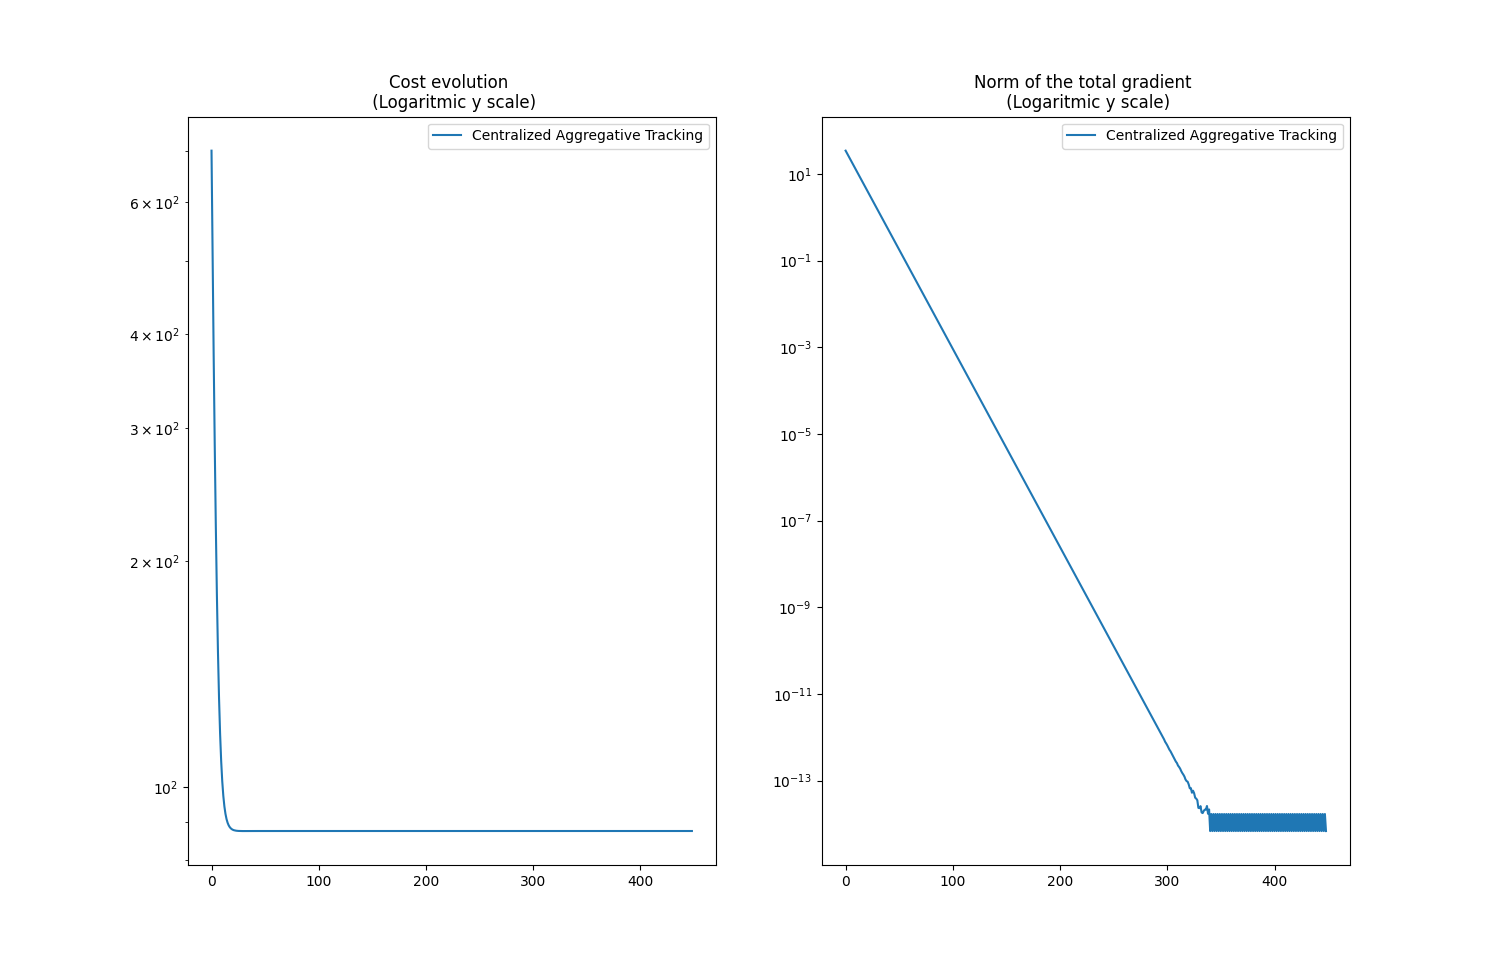
\includegraphics[width=0.8\linewidth]{report/figs/centralized_agt.png}
    \caption{Centralized aggregative optimization applied to a team of four agents. The figure illustrates fast consensus convergence and the linear decrease of the gradient norm toward zero.}
\end{figure}
As illustrated, the centralized algorithm behaves as expected: the agents quickly reach consensus on a common configuration, and the norm of the gradients converges linearly to zero.

\medskip
\paragraph{Distributed setting.}
Let us now proceed with the distributed algorithm.  
As mentioned in the previous section, in distributed scenarios each agent lacks access to the full network data, making it impossible to compute the gradient exactly as in the centralized case. To overcome this, we rely on local proxy variables \(s_i^k\) and \(v_i^k\) that track the global aggregative quantities in a decentralized manner.   \\
Recall that the distributed aggregative tracking optimization algorithm is defined by the following update rules:
\begin{align*}
z_i^{k+1} &= z_i^k - \alpha \left( \nabla_1 \ell_i(z_i^k, s_i^k) + \nabla \phi_i(z_i^k) v_i^k \right), & z_i^0 &\in \mathbb{R}^{n_i} \\
s_i^{k+1} &= \sum_{j \in \mathcal{N}_i} a_{ij} s_j^k + \phi_i(z_i^{k+1}) - \phi_i(z_i^k), & s_i^0 &= \phi_i(z_i^0) \\
v_i^{k+1} &= \sum_{j \in \mathcal{N}_i} a_{ij} v_j^k + \nabla_2 \ell_i(z_i^{k+1}, s_i^{k+1}) - \nabla_2 \ell_i(z_i^k, s_i^k), & v_i^0 &= \nabla_2 \ell_i(z_i^0, s_i^0)
\end{align*}
Here, each agent \(i\) updates its estimate \(z_i\) based on local gradients evaluated at the proxy variables, while \(s_i\) and \(v_i\) evolve through weighted consensus steps over neighbors \(\mathcal{N}_i\), combined with local corrections to track the global aggregative quantities and their gradients. 

\noindent The following figure (Figure \ref{fig:distributed_agt})  shows the same scenario as the centralized aggregative optimization simulation, but now the agents communicate over a random graph.

\newpage
\begin{figure}[h!]
    \centering
    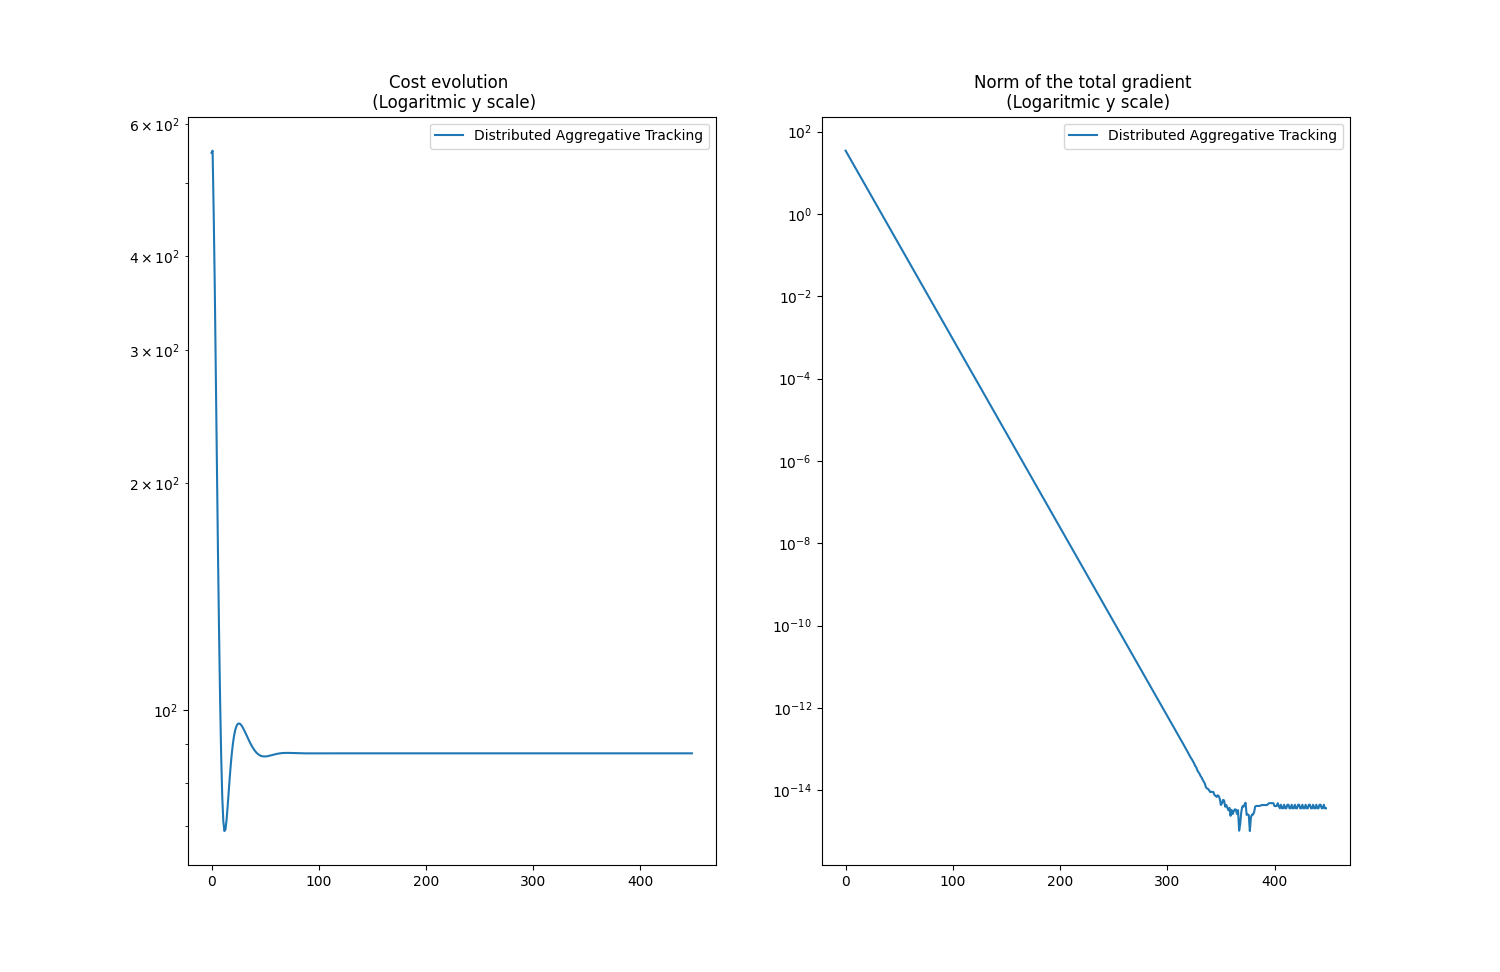
\includegraphics[width=0.7\linewidth]{report/figs/distributed_agt.png}
    \caption{Results of the Distributed Aggregative Optimization Algorithm}
    \label{fig:distributed_agt}
\end{figure}
\noindent Also in this case, the convergence theorem holds, and the norm of the gradient converges to zero at a linear rate.

\begin{figure}[h!]
  \centering
  \begin{minipage}{0.5\textwidth}
    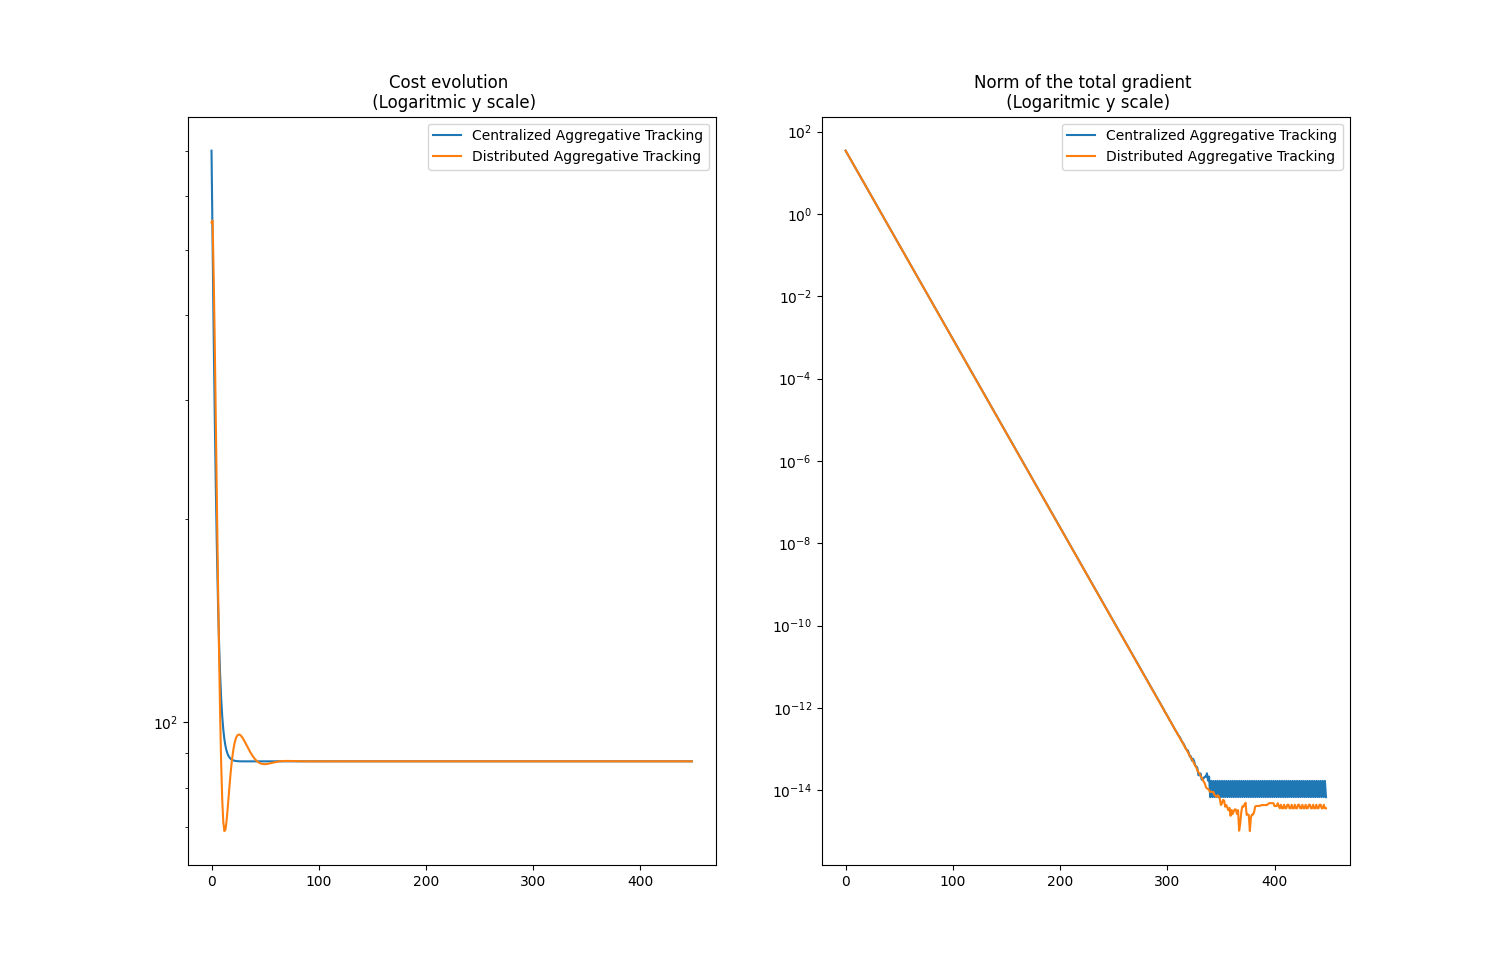
\includegraphics[width=\linewidth]{report/figs/comparison_centr_disp_agt.png}
  \end{minipage}%
  \hfill
  \begin{minipage}{0.5\textwidth}
    \small
    The plot compares the convergence behavior of both the centralized and distributed algorithms. As expected, both satisfy the convergence theorem. The distributed algorithm experiences slower convergence due to the limited local communication among agents-each agent only communicates with its neighbors. However, after a sufficient number of iterations, consensus is reached across the network.
  \end{minipage}
  \caption{Comparison of Convergence between Distributed and Centralized Aggregative Optimization Algorithms}
\end{figure}

\paragraph{Simulations}
To better understand the effectiveness of our implementation, we tested the same algorithm under different conditions by varying both the graph topology and the agents' behaviors. In particular, we considered three scenarios that highlight different trade-offs between individual objectives and aggregative terms. \\
In the first scenario (Figure \ref{fig:vip}) , we introduced a ``VIP" agent that does not follow a specific target, but is constrained to remain close to the barycenter of all agents. This can be interpreted as a situation where the rest of the agents must coordinate to ``protect'' the VIP. 

\newpage 
\begin{figure}[h!]
  \begin{minipage}{0.50\textwidth}
    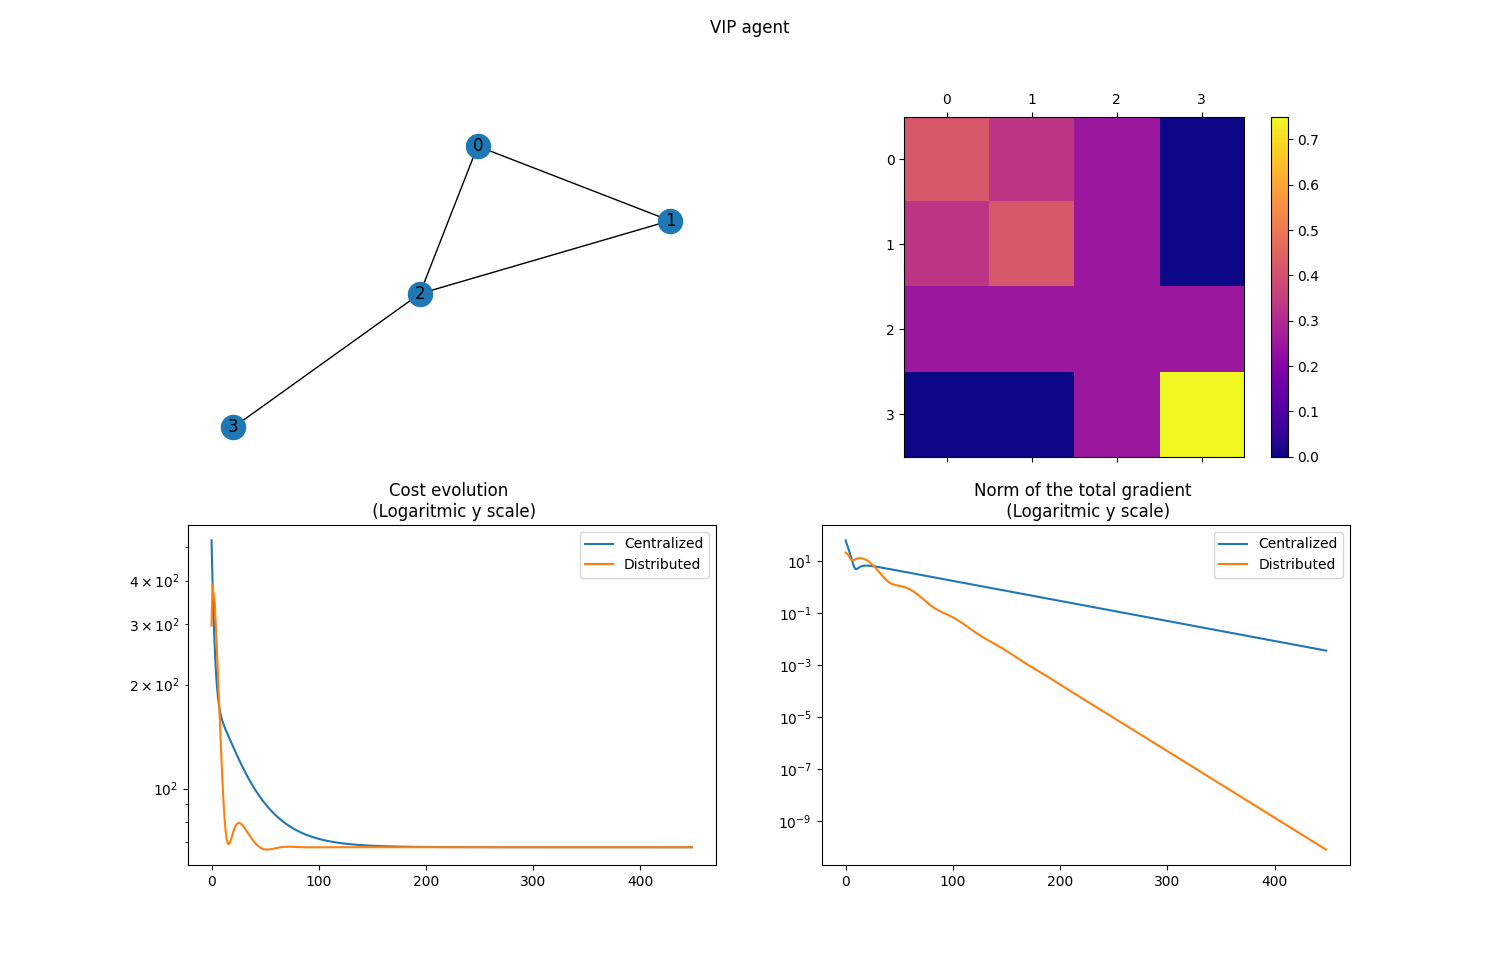
\includegraphics[width=\linewidth]{report/figs/VIP_agent.png}
  \end{minipage}%
  \hfill
  \begin{minipage}{0.50\textwidth}
    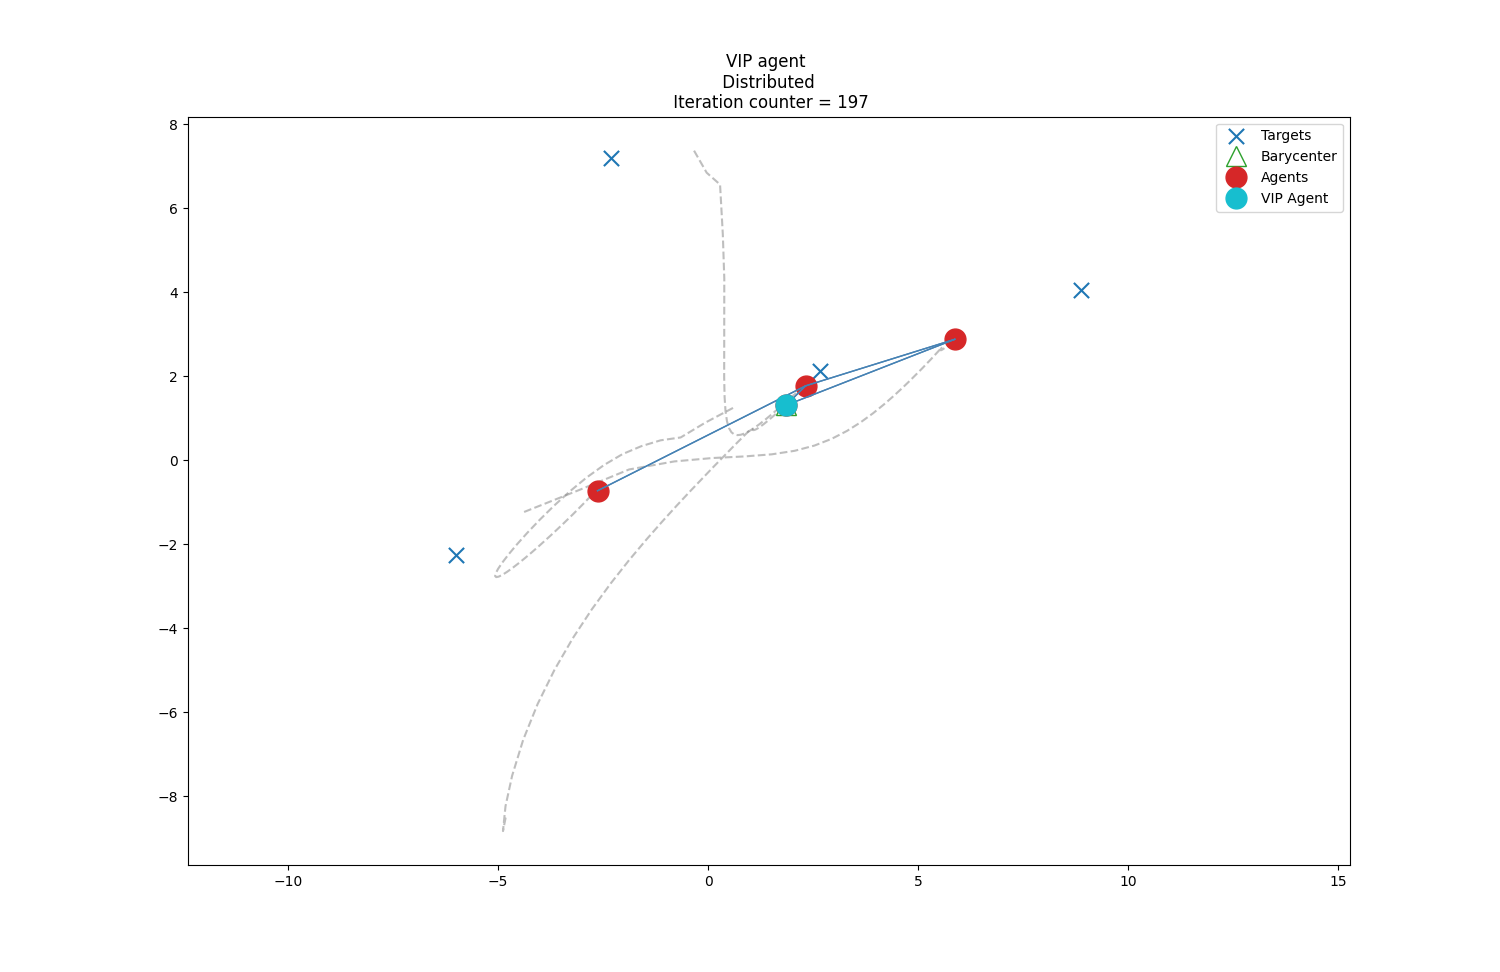
\includegraphics[width=\linewidth]{report/figs/VIP_agent_Distributed.png}
  \end{minipage}
  \caption{Aggregative tracking with VIP agent fixed at the barycenter.}
  \label{fig:vip}
\end{figure}

In the second scenario (Figure \ref{fig:team_cohesion}), we increased the weight of the aggregative term in each cost function. In this case, the agents prioritize staying close to one another rather than to their individual targets. This promotes group cohesion and leads to tightly clustered trajectories, often at the expense of accuracy in target tracking.

\begin{figure}[h!]
  \begin{minipage}{0.50\textwidth}
    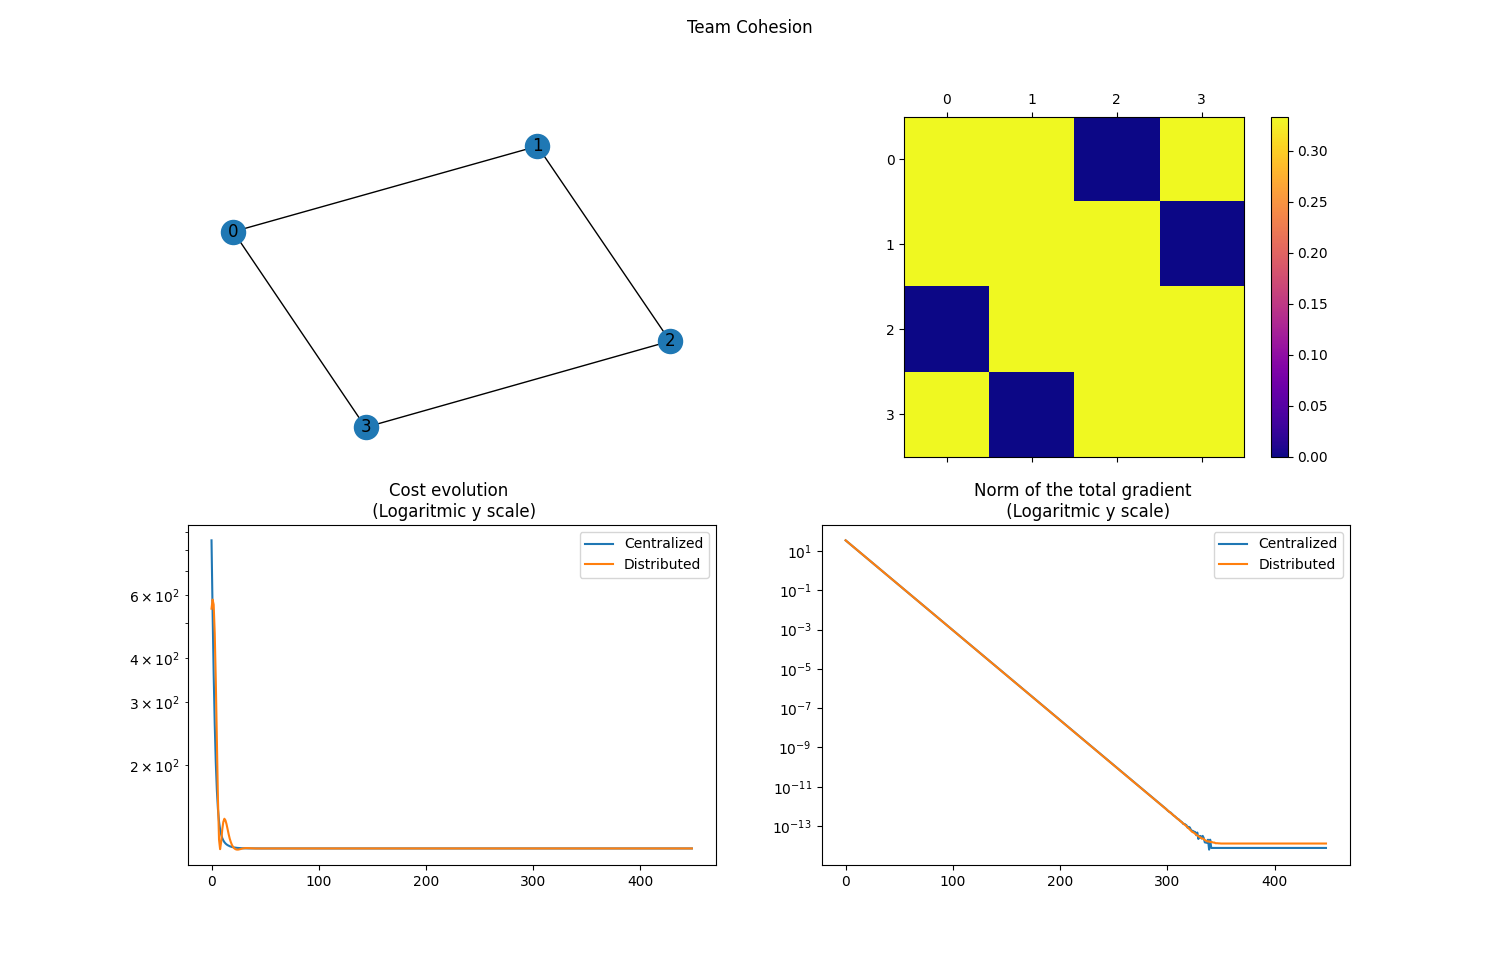
\includegraphics[width=\linewidth]{report/figs/Team_Cohesion.png}
  \end{minipage}%
  \hfill
  \begin{minipage}{0.50\textwidth}
    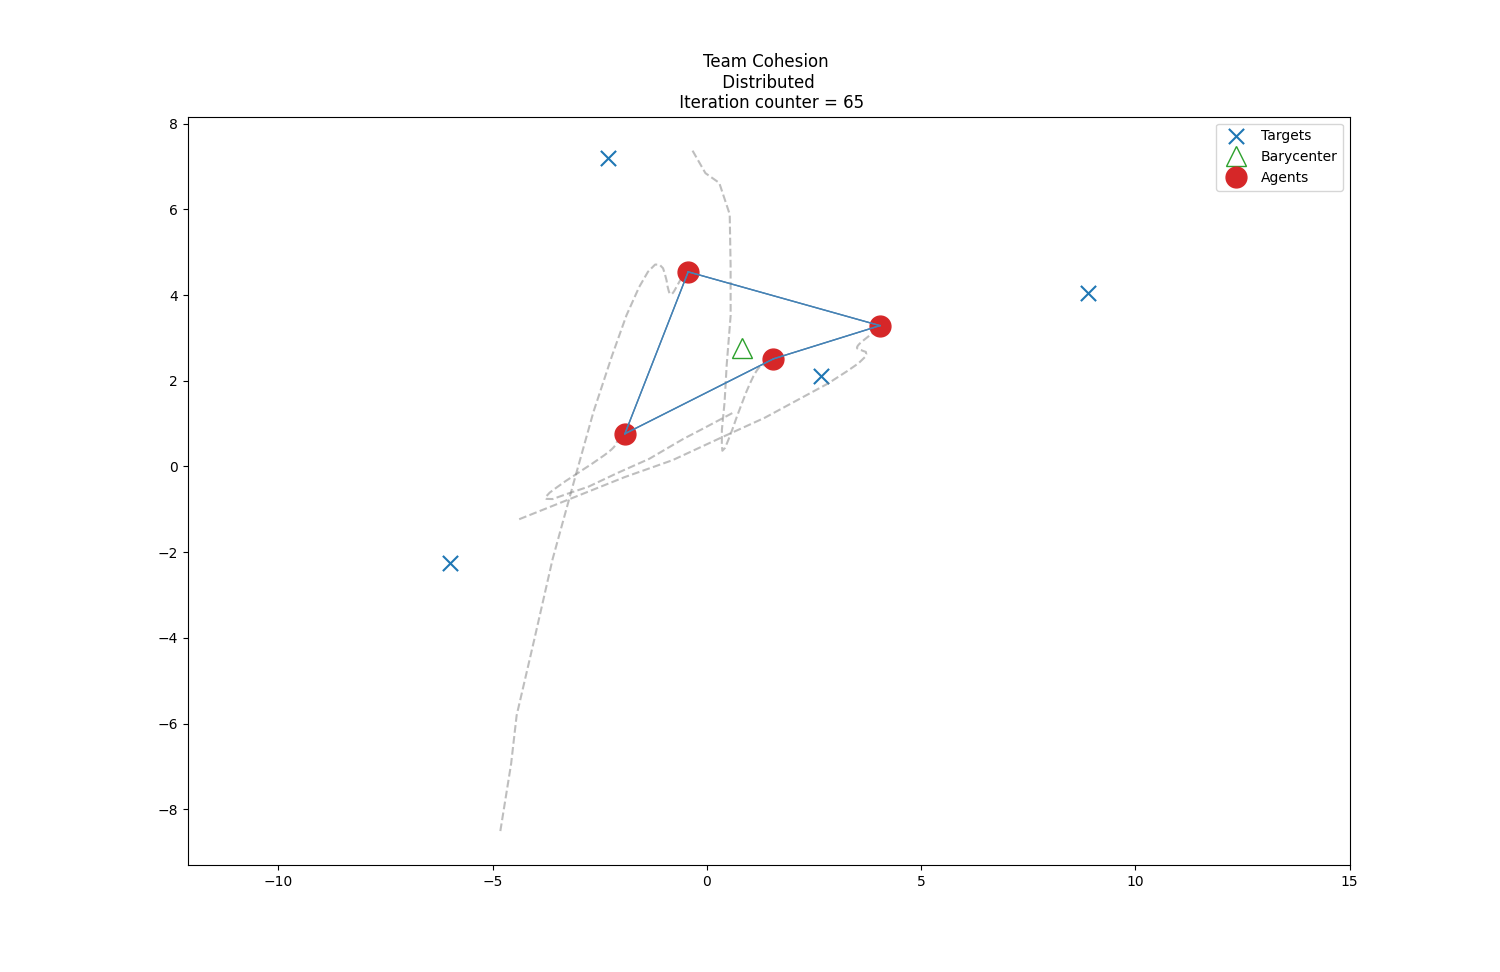
\includegraphics[width=\linewidth]{report/figs/Team_Cohesion_Distributed.png}
  \end{minipage}
  \caption{Aggregative tracking with stronger team cohesion.}
  \label{fig:team_cohesion}
\end{figure}

Finally, we considered the opposite setting, where agents are driven more strongly by their private targets and less influenced by the aggregative term (Figure \ref{fig:closer_target}). This results in trajectories that more closely follow the desired target paths, while still maintaining some degree of coordination.

\begin{figure}[h!]
  \begin{minipage}{0.50\textwidth}
    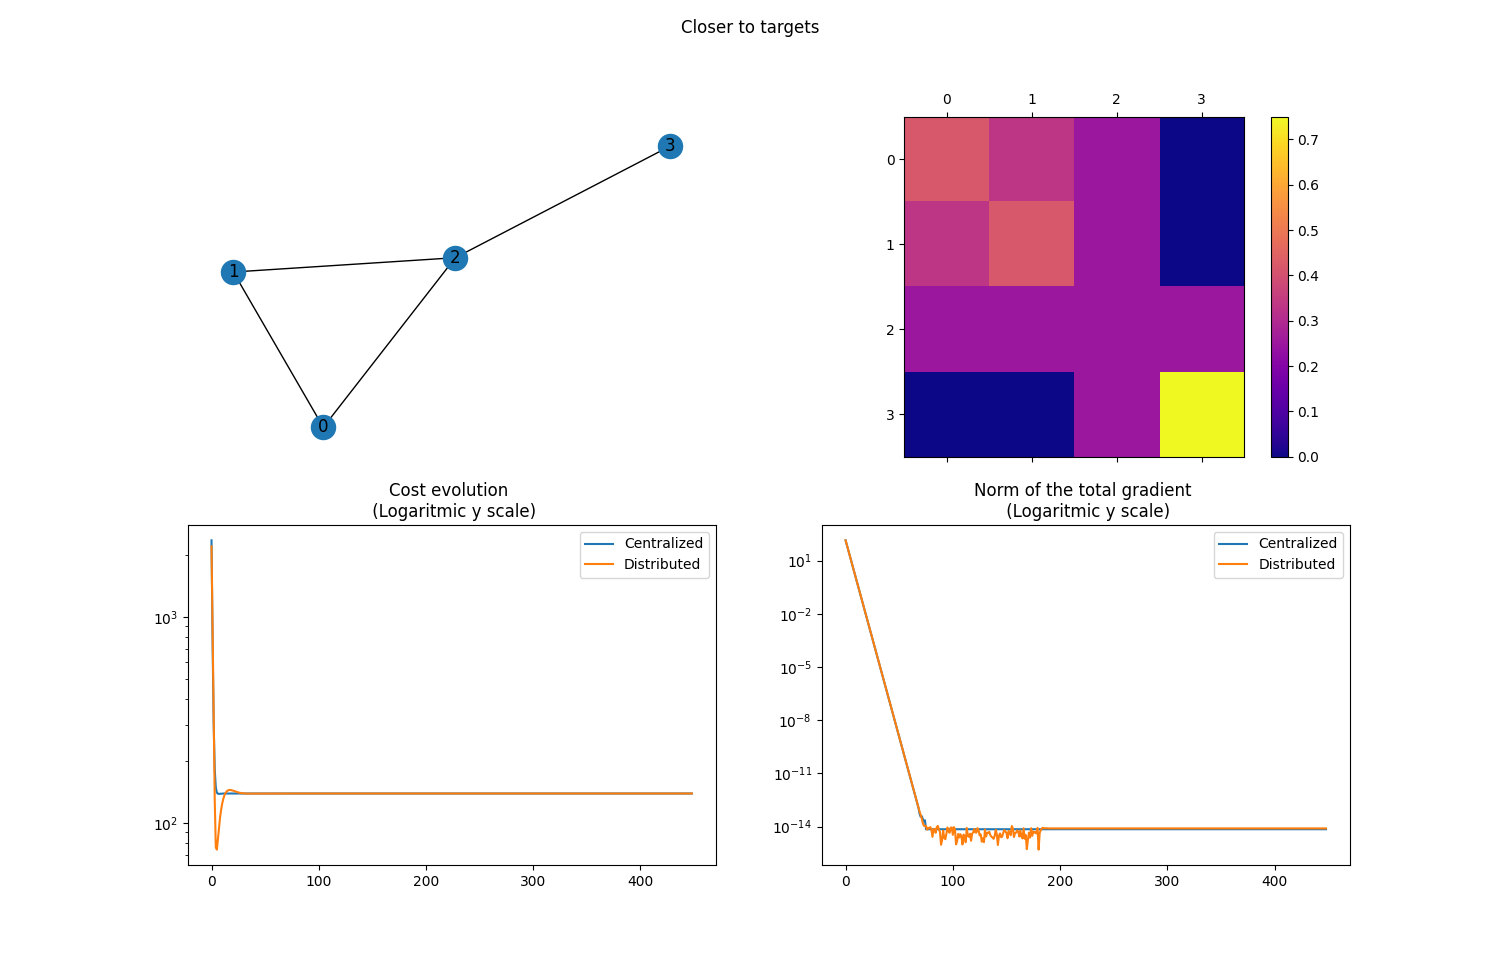
\includegraphics[width=\linewidth]{report/figs/Closer_to_targets.png}
  \end{minipage}%
  \hfill
  \begin{minipage}{0.50\textwidth}
    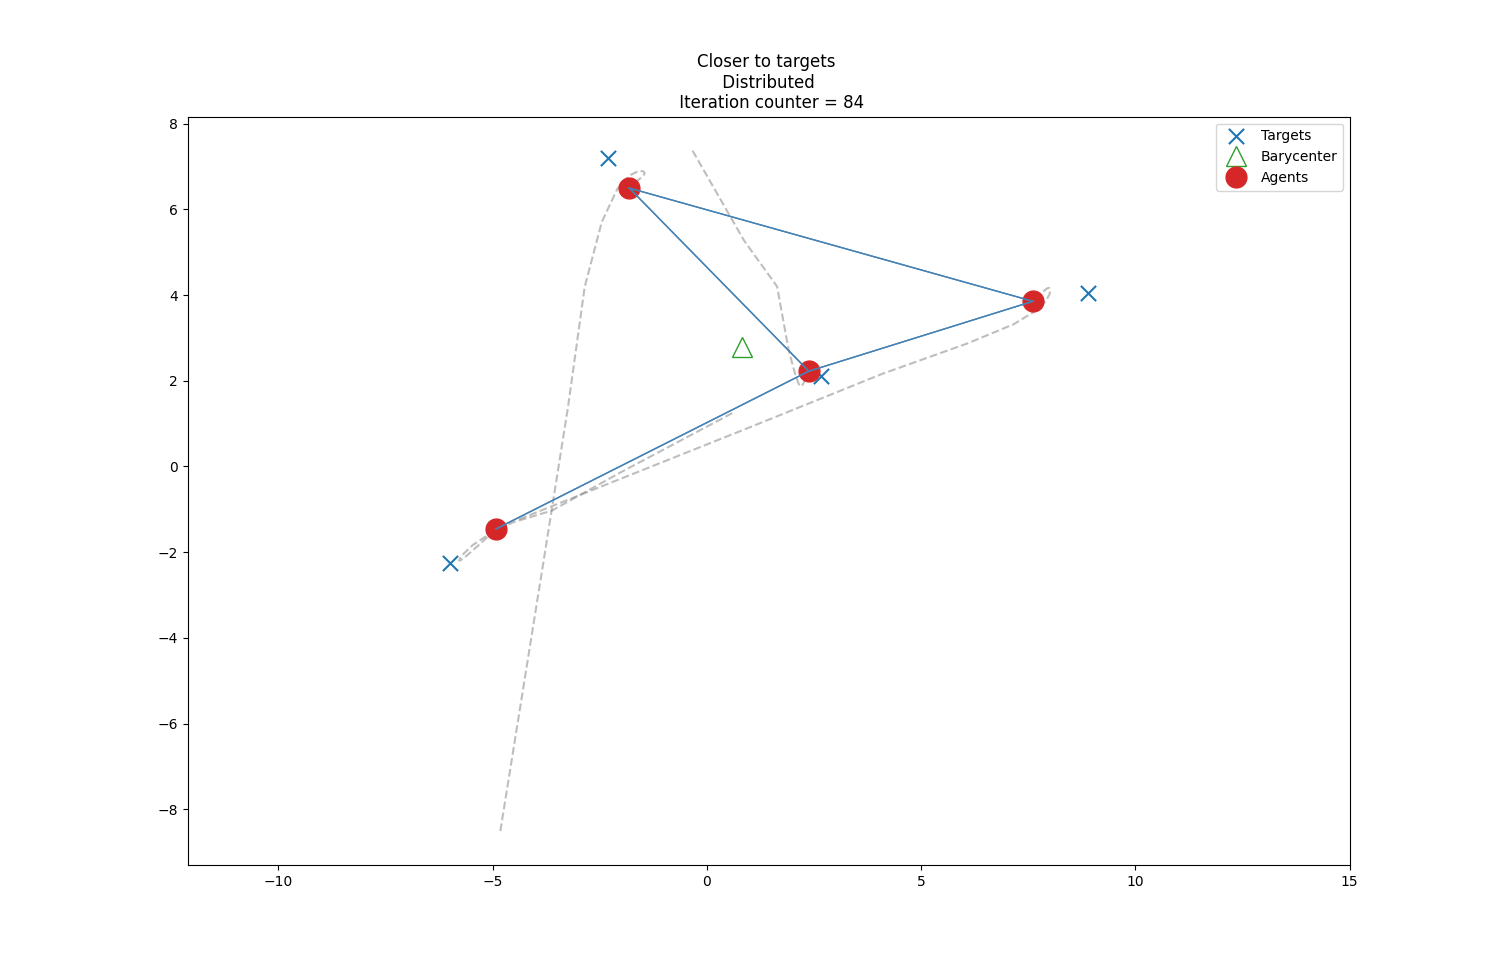
\includegraphics[width=\linewidth]{report/figs/Closer_to_targets_Distributed.png}
  \end{minipage}
  \caption{Aggregative tracking with stronger focus on individual targets.}
  \label{fig:closer_target}
\end{figure}

\newpage

\subsection{Aggregative Tracking Distributed Optimization Algorithm with a Low-Level Multi-Robot Safety Controller}
\label{sec:collision_avoidance}

The cooperative aspect of multi-robot control corresponds to a high-level task that focuses on achieving collective objectives, such as formation control, coverage, or task allocation. This is fundamentally different from obstacle avoidance, which is considered a lower-level task concerned primarily with ensuring the safety of each individual robot by preventing collisions with obstacles or other robots. \\
In this context, a safety controller used on a distributed algorithm can be interpreted as a safety filter. Its role is to adjust or modify the control inputs generated by the high-level cooperative controller in real time, so as to guarantee collision avoidance and maintain safe operation of the robotic team. By filtering the reference inputs, the safety controller ensures that safety constraints are respected without compromising the overall cooperative behavior, thereby smoothly integrating high-level coordination with low-level safety.


\begin{center}
\begin{tikzpicture}[
    block/.style={rectangle, draw, rounded corners, minimum width=5cm, minimum height=1.2cm, align=center},
    >=Stealth
]

% Blocks
\node[block] (dist) {Distributed Algorithm};

% Middle block
\node[block, below=0.5cm of dist] (safety) {Safety Controller};

% Arrow from dist to safety
\draw[->] (dist.south) -- node[right, xshift=2mm]{$u^{\mathrm{REF}}(x)$} (safety.north);

% Lower block
\node[block, below=0.5cm of safety] (actuators) {
    Actuators \\
    $\dot{x}(t) = f(x(t)) + g(x(t)) \cdot u(t)$
};

% Arrow from safety to actuators
\draw[->] (safety.south) -- node[right, xshift=2mm]{$u(t) = \kappa(x)$} (actuators.north);

\end{tikzpicture}
\end{center}

\paragraph{Safety Control for Multi-Robot Systems}

The main idea of the safety control is to separate the safe and unsafe areas via a single function, which differs only in sign:
\[
V^s(x) \geq 0 \quad \text{(safe)}, \qquad V^s(x) < 0 \quad \text{(unsafe)}.
\]
Our goal is to design a control law such that if the system state is in the safe set initially, it remains there for all future time (forward invariance).  \\
Formally, if we consider a control-affine nonlinear dynamical system:
\[
\dot{x}(t) = f(x(t)) + g(x(t)) u(t), \quad t \geq 0,
\]
with state $x \in \mathbb{R}^n$ and control input $u \in U \subset \mathbb{R}^m$.

Define the safe state set
\[
\mathcal{X}^s := \{ x \in \mathcal{X} \subset \mathbb{R}^n \mid V^s(x) \geq 0 \}
\]
for some sufficiently regular function
\[
V^s : \mathcal{X} \subset \mathbb{R}^n \to \mathbb{R}.
\]
The goal is to design a feedback control law $\kappa^s : \mathcal{X} \to \mathbb{R}^m$ such that $\mathcal{X}^s$ is forward invariant, i.e., any trajectory starting in $\mathcal{X}^s$ at $t=0$ remains in $\mathcal{X}^s$ for all $t \geq 0$.

\medskip
Let's now focus on the case of multi-robot collision avoidance. \\
Consider a team of $N$ robots modelled as single integrators, i.e., for $i = 1, \ldots, N$,
\[
\dot{x}_i = u_i,
\]
with $x_i \in \mathbb{R}^d$ the state (position) of robot $i$ and $u_i \in U \subset \mathbb{R}^d$ the control input.
Out goal is to keep the robots at a safe distance $\Delta > 0$ from each other.
% For simplicity, consider scalar states and inputs: $x_i, u_i \in \mathbb{R}$ and $U \equiv \mathbb{R}$. \\
Consider the time derivative of $V^s(x(t))$ along the system trajectories
\begin{align*}
\frac{d}{dt} V^s(x(t)) &= \nabla V^s(x(t))^\top f(x(t)) + \sum_{h=1}^m \nabla V^s(x(t))^\top g_h(x(t)) u_h(t) \\
&= L_f V^s(x(t)) + L_g V^s(x(t)) u(t),    
\end{align*}
For the single integrator system, we have
\[
f(x(t)) = 0, \quad g(x(t)) = I,
\]
thus
\[
\frac{d}{dt} V^s(x(t)) = \nabla V^s(x(t))^\top u(t) = L_gV^s(x(t)) u(t) 
\]

We say that $V^s$ is a Control Barrier Function if there exists a continuous, strictly increasing function $\gamma : \mathbb{R} \to \mathbb{R}$ with $\gamma(0) = 0$ such that
\[
\sup_{u \in U} \left[ L_f V^s(x) + L_g V^s(x) u + \gamma\bigl(V^s(x)\bigr) \right] \geq 0.
\]
The above inequality induced by a Control Barrier Function is called a Control Barrier Certificate. \\
Note that the condition allows the time derivative of \( V^s(x) \) to be negative of a certain amount depending on the distance from the boundary defined by \( V^s(x) = 0 \). The crucial aspect is that the function \( \gamma \) is strictly increasing: this ensures that, if the system starts in the unsafe region (i.e., \( V^s(x) < 0 \)), the dynamics are driven toward the safe set \( \{ x \mid V^s(x) \geq 0 \} \); once the state reaches the safe set (i.e., \( V^s(x) \geq 0 \)), the condition guarantees forward invariance.

Going back to multi-robot collision avoidance problem, let's consider a pair-wise local CBF defined as
\[
V^s_{i,j}(x_i, x_j) = \|x_i - x_j\|^2 - \Delta^2,
\]
where $\Delta$ denotes the safety distance between robots $i$ and $j$.

The gradients are
\[
\nabla_1 V^s_{i,j}(x_i, x_j) = 2(x_i - x_j), \quad \nabla_2 V^s_{i,j}(x_i, x_j) = 2(x_j - x_i),
\]
where $\nabla_1 V^s_{i,j}(\cdot, \cdot)$ represents the gradient of $V^s_{i,j}$ with respect to the first variable and $\nabla_2 V^s_{i,j}(\cdot, \cdot)$ represents the gradient of $V^s_{i,j}$ with respect to the second variable. Gradient w.r.t.\ all other states is zero.

Let $u \in \mathbb{R}^{dN}$ be the stacked input vector for all $N$ robots.

The admissible control space for collision avoidance is obtained by intersecting all pair-wise control barrier certificate constraints:
\begin{align*}
    \mathcal{U}^s(x) &= \left\{ u \in \mathbb{R}^{dN} \mid 
    -\nabla_1 V^s_{i,j}(x_i, x_j)^\top u_i - \nabla_2 V^s_{j,i}(x_j, x_i)^\top u_j - \gamma V^s_{i,j}(x_i, x_j) \leq 0, \right. \\
    & \quad \left. \forall i \in \{1,\ldots,N\}, \quad \forall j \in \mathcal{N}_i \right\}.
\end{align*}
where $\mathcal{N}_i$ includes all robots $j$ that may collide with robot $i$. \\
It is worth noting that, in this case, the strictly increasing function \( \gamma \) is chosen as a linear function, \( \gamma(x) = \gamma \cdot x \). The parameter \( \gamma > 0 \) governs the conservativeness of the resulting constraint: a larger value of \( \gamma \) allows \( V^s(x) \) to attain more negative values even near the boundary \( V^s(x) = 0 \), thereby permitting the agents to pass closer to each other. Conversely, a smaller value of \( \gamma \) results in more conservative behavior, maintaining a greater safety margin. 

\medskip
Let's now define the safety controller for multi-robot collision avoidance in the distributed scenarios.
As we already know, in distributed multi-robot scenarios, it is desirable to avoid a central coordinator, so we will need a more constrained problem formulation. \\
Let $u_{\mathrm{ref}}(x) \in \mathbb{R}^d$ be a (possibly unsafe) reference input, e.g., from a higher-level controller.  
The safety controller is designed to be minimally invasive, i.e., to modify the reference input as little as possible. \\
So, the safe control policy $u_i = \kappa_i^s(x)$ can be designed as:
\[
\kappa^s_i(x) = \arg\min_{u_i \in \mathbb{R}^d} \|u_i - u_i^{\mathrm{ref}}\|^2
\]
subject to
\begin{align*}
    -\nabla_1 V^s_{i,j}(x_i, x_j)^\top u_i - \tfrac{1}{2} \gamma (V^s_{i,j}(x_i, x_j)) \leq 0,  \\ 
    \quad \|u_i\| \leq u_i^{\max}, \quad \forall j \in \mathcal{N}_i. 
\end{align*}

The $\frac{1}{2}$ is introduced to symmetrically split the degree of freedom between the two agents involved, $i$ and $j$.

\subsubsection{Our Implementation of Safety Controller}
In this section, we explore a practical approach to safety control in distributed multi-robot scenarios, focusing on how agents locally detect and avoid collisions while maintaining coordinated behavior.

\medskip
First of all, we need to define a function that identifies the physical neighbors of each agent. As an implementation choice, we compute this information in a semi-centralized manner: every time an agent needs to determine its next state, a function is called to compute the distances to all other agents and return only those that fall within a predefined radius \( r \), thus identifying its actual neighbors. While this approach simplifies the implementation, it is not suitable for real-world distributed systems, where no centralized unit is available to compute global distances. However, it can be interpreted in a distributed context as each agent being equipped with sensors such as LiDAR that provide real-time distance measurements to nearby agents and obstacles.

\medskip
Once the distances from neighbors are obtained, the agent computes its next state using a safety controller. This controller takes as input the desired control action computed by the high-level distributed aggregative algorithm. Since the system is modeled with single-integrator dynamics, the output of the aggregative controller is first processed by a proportional (P) controller, which generates a control signal compatible with the assumed dynamics. The safety controller then solves a constrained optimization problem to ensure safety and sends the resulting safe control input to the actuators. The outcome is also fed back to the high-level controller to maintain an accurate estimate of the agent's state, effectively closing the loop with a feedback mechanism.

\medskip
In certain scenarios, particularly when the environment becomes too crowded, we observed that the optimization problem might become infeasible due to excessive constraints. To address this, we implemented a simple fallback mechanism: if the optimization problem cannot be solved, the agent stops. This behavior introduces a form of implicit priority or ``right-of-way" mechanism, where agents wait until it is safe to move again, preventing collisions while still allowing eventual progress.

\medskip
Once the agents have resolved their local interactions and reached a safe configuration, the safety controller allows the control input from the high-level controller to pass through to the actuators in a linear fashion. As a result, the system retains the same convergence properties as the original aggregative distributed algorithm in the absence of safety concerns.

\begin{figure}[H]
  \begin{minipage}{0.5\textwidth}
    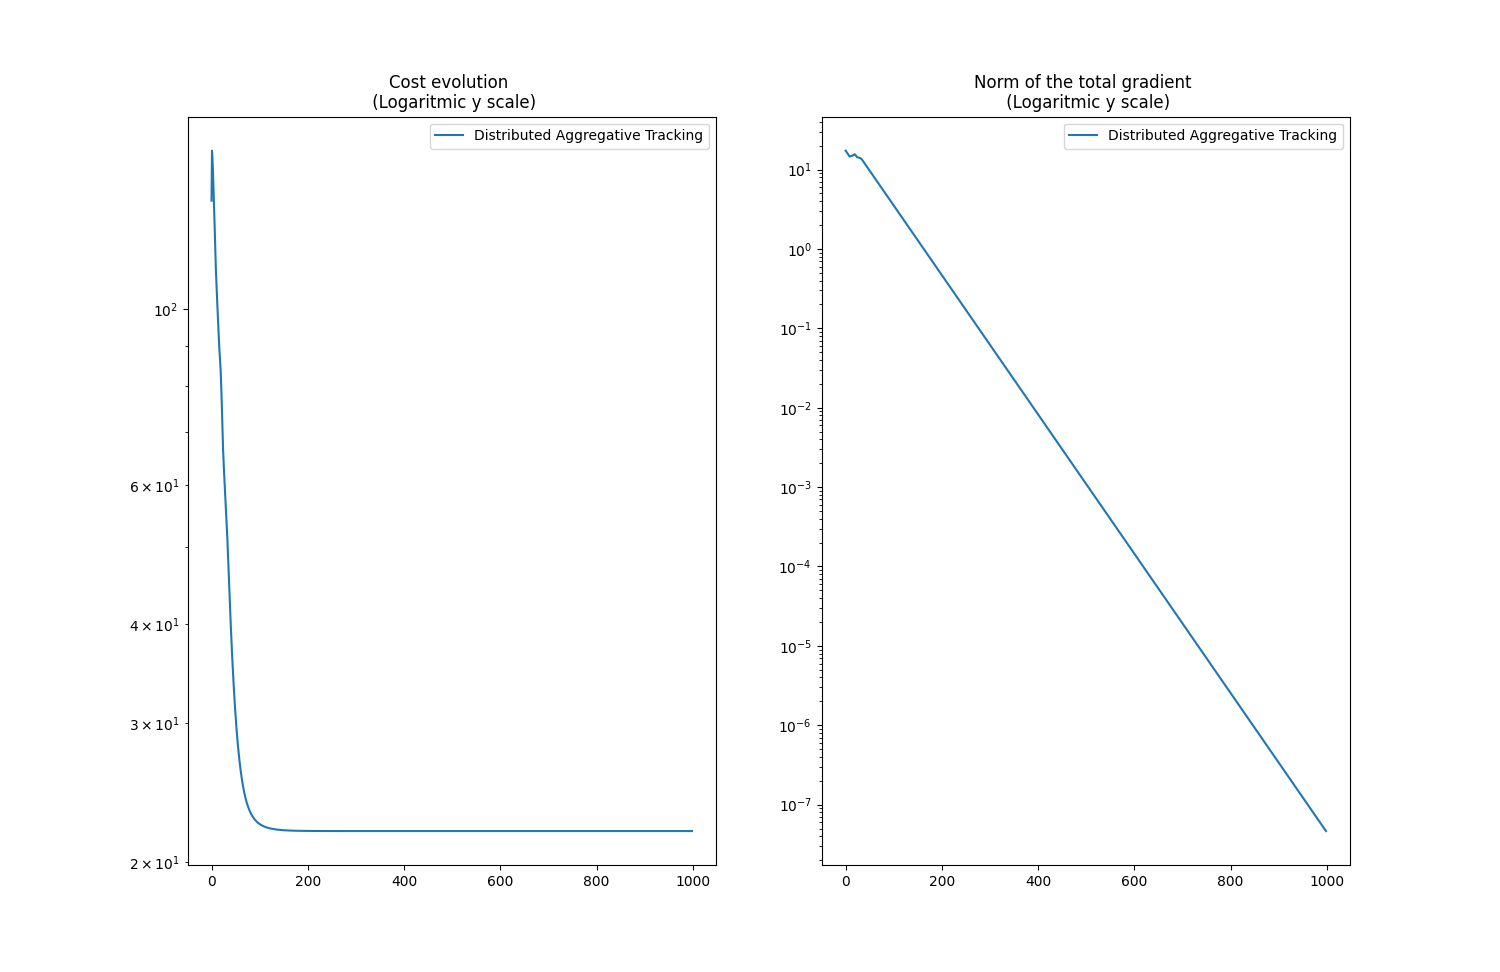
\includegraphics[width=\linewidth]{report/figs/safety_contr.png}
  \end{minipage}%
  \hfill
  \begin{minipage}{0.5\textwidth}
    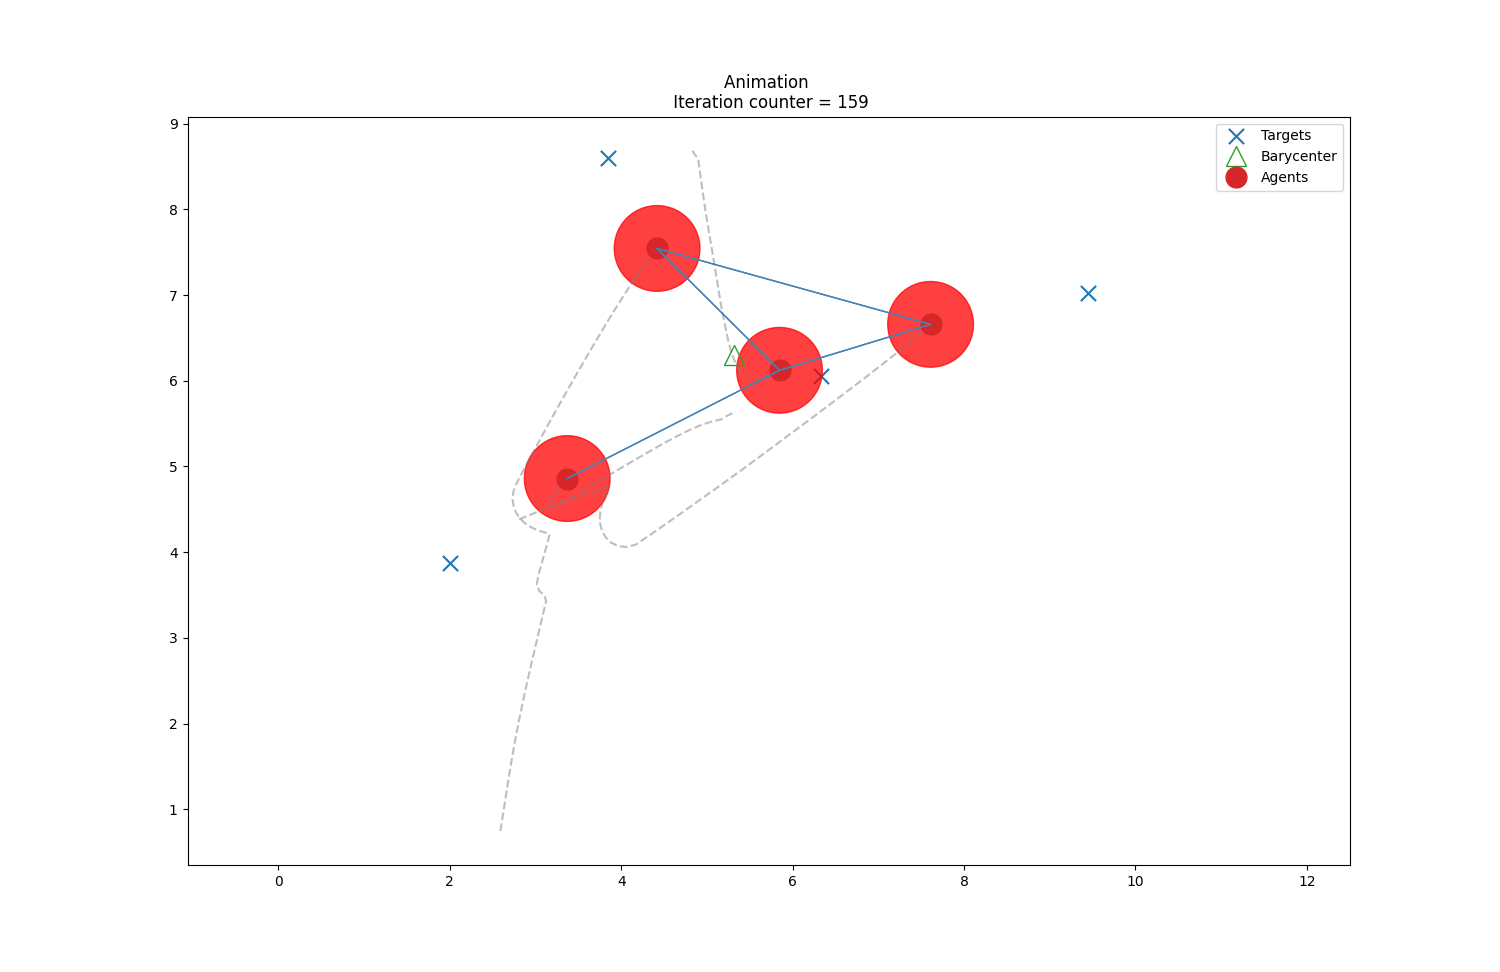
\includegraphics[width=\linewidth]{report/figs/safety_animation.png}
  \end{minipage}%
  \caption{Safety controller performance in multi-robot collision avoidance. In the animation (image on the right), it is possible to see a red circle which represents the unsafe collision area of each agent.}
  \label{fig:rviz_result}
\end{figure}

This structure is particularly interesting because it clearly acts as a low-level safety mechanism: the higher-level controller is unaware of its presence, and yet the safety layer operates seamlessly in the background for each agent.

\medskip
While the proposed approach provides an effective and practical method for implementing a safety controller in multi-robot systems, several limitations may arise in more complex scenarios. In particular, accounting for dynamic constraints and input bounds can lead to infeasibility of the optimization problem, making it impossible to guarantee safety under all conditions. Furthermore, when the objectives of multiple agents conflict with the safety barrier constraints, the system may experience deadlocks. These challenges highlight the need for more sophisticated control strategies that ensure both safety and feasibility in distributed multi-agent systems.

\newpage

\section{Aggregative Tracking Implemented with ROS2 Framework}

Robot Operating System (ROS) is an open-source framework designed to support the development, integration, and management of software for robotic systems. It simplifies how different components of a robot such as sensors, actuators, and control modules communicate and coordinate, even when these components are distributed across multiple machines. \\
In ROS, each functional unit is implemented as an independent node, which performs specific tasks like reading sensor data, computing control commands, or logging information. Communication between nodes occurs through named data channels called topics. Nodes publish data to topics or subscribe to receive data from them. This publish-subscribe model supports anonymous and decoupled communication: nodes do not require direct knowledge of one another, but instead communicate indirectly through the shared topic namespace. \\
This modular and distributed architecture is particularly well-suited to multi-agent systems. In the context of distributed optimization, the publish-subscribe model naturally maps to a communication graph, where each agent exchanges data only with its immediate neighbors. For example, if an agent subscribes to a topic published by another agent, the publisher is considered its in-neighbor. Conversely, if it publishes data read by others, it is an out-neighbor. This mapping allows each agent to maintain private local data while interacting only with nearby agents, following the typical assumptions of distributed algorithms and enabling scalable, decentralized coordination. \\
Each agent begins by extracting its configuration parameters, such as the communication graph structure and adjacency matrix, from a predefined launch file. These parameters are not computed dynamically, but are instead initialized before execution, and can be considered centralized information that is locally known by each agent at runtime. \\
Once initialized, the agent operates in a fully distributed manner. It publishes two types of information: its internal state, defined by the variables \( z \), \( s \), and \( v \); and auxiliary data used for logging and visualization. Simultaneously, it subscribes to the state topics of its neighbors, receiving only the information required by the algorithm. This setup ensures that each agent communicates only with its local neighborhood. Moreover, because the communication graph includes self-loops, each agent also subscribes to its own topic, processing its data through the same interface as data from others. \\
To maintain temporal consistency and synchronization, each agent uses a timer-based callback mechanism triggered every 0.1 seconds. During each callback, the agent checks whether it has received the latest state data from all of its neighbors. Once all the necessary data have been collected in a queue, the agent proceeds to update its estimate of \( z \) and the auxiliary variables \( s \) and \( v \). This ensures that updates occur only when all dependencies are satisfied, providing a synchronized and consistent evolution of the distributed algorithm. \\
The distributed algorithm implemented is an aggregative tracking scheme, as described in Section \ref{sec:dist_aggr}. This algorithm enables each agent to update its local state based only on the data received from its immediate neighbors. As a result, the overall system behaves in a fully distributed manner, where coordination emerges from local interactions without any central controller.

\begin{figure}[H]
    \centering
    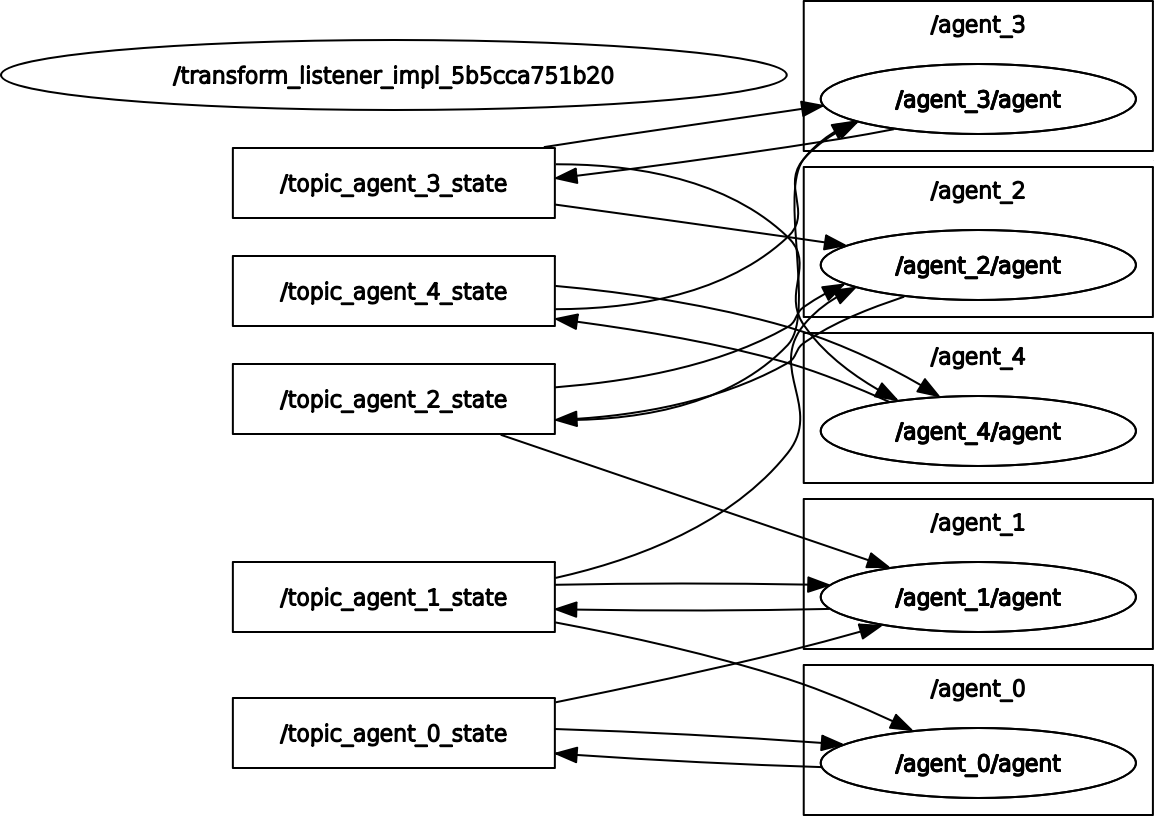
\includegraphics[width=0.6\linewidth]{report/figs/rosgraph_topics_agents.png}
    \caption{ROS graph structure showing the topic connections between agents, the subscriptions are determined using a Erd\H{o}s--R\'enyi communication graph with edge probability $p = 0.65$. Note: the self-loops are modelled with self-subscriptions.}
\end{figure}

Simultaneously, a dedicated visualizer node is responsible for aggregating and rendering the system state in real time using RViz. RViz is a three-dimensional visualization tool designed for robotic applications. It can display robot models, sensor data, and environmental elements using a rich set of plugins. \\
The visualizer subscribes to two topics for each agent: one containing the agent's position and internal state (topic\_agent\_i\_state), and the other containing performance metrics such as the cost and gradient norm (topic\_agent\_i\_plot\_info). Incoming messages are buffered in FIFO queues to enable synchronized data processing. \\
As with the agents, a timer callback is executed periodically. At each time step, the visualizer checks for synchronized data from all agents. Once data synchronization is ensured, the visualizer executes several tasks. It publishes the positions of all targets, computes and publishes the total cost and the norm of the aggregated gradient, and renders the positions of all agents along with their barycenter. These values are visualized in RViz to provide a real-time, intuitive representation of the system's evolution and performance.


\begin{figure}[H]
  \begin{minipage}{0.45\textwidth}
    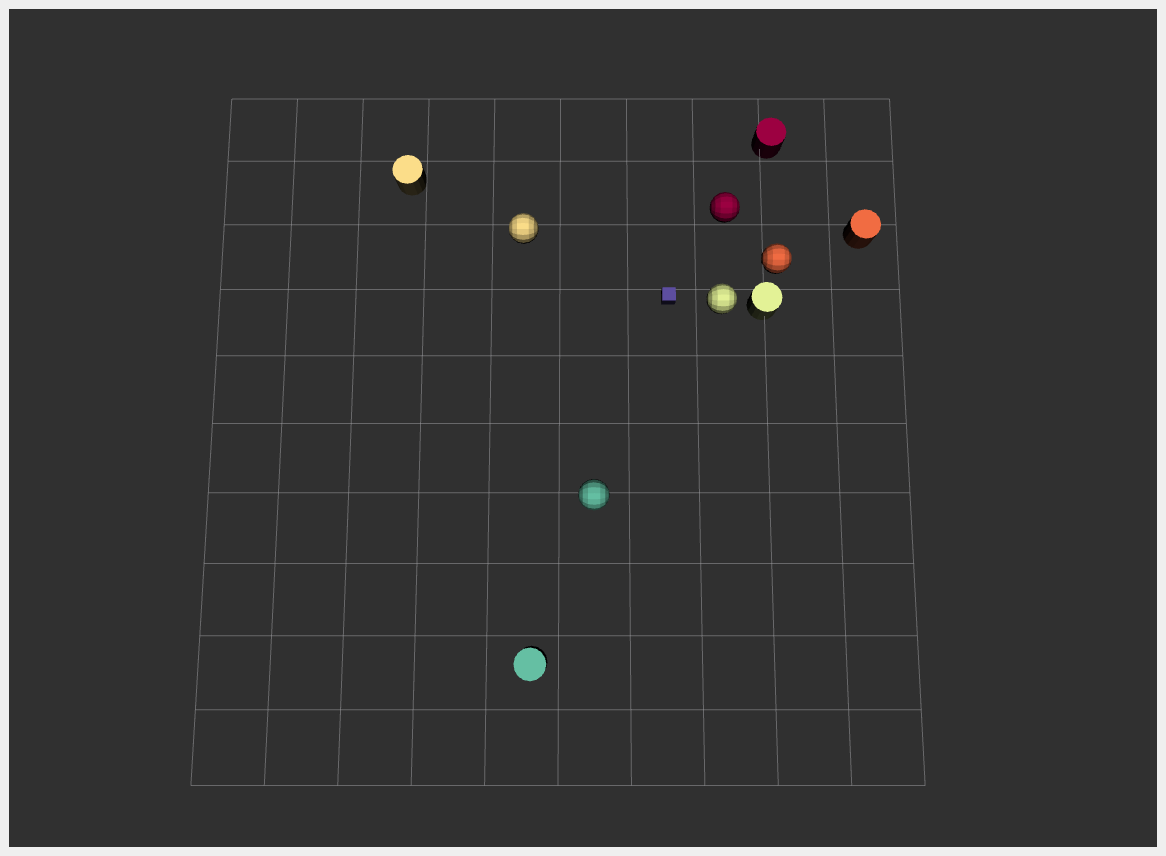
\includegraphics[width=\linewidth]{report/figs/result_rviz.png}
  \end{minipage}%
  \hfill
  \begin{minipage}{0.45\textwidth}
    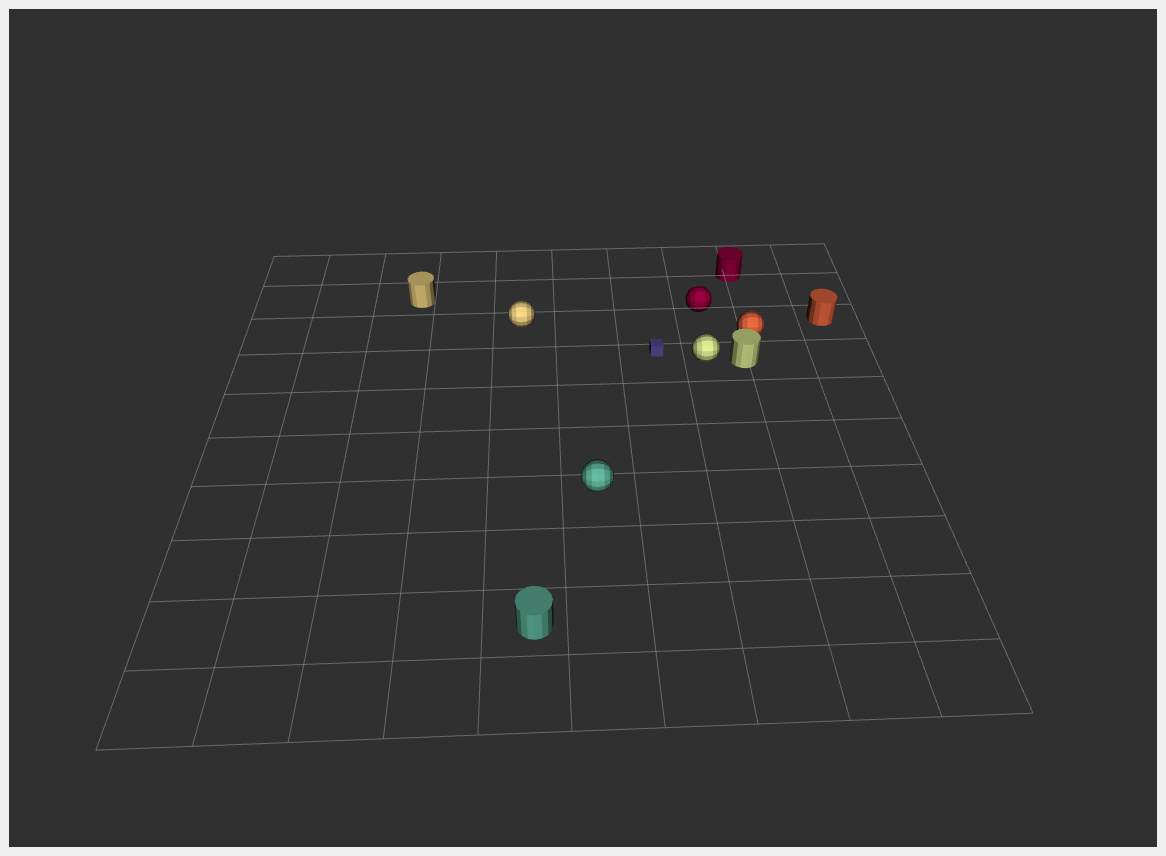
\includegraphics[width=\linewidth]{report/figs/rviz_result_2.png}
  \end{minipage}%
  \caption{Visualization of agent positions in RViz.}
  \label{fig:rviz_result}
\end{figure}

\begin{figure}[H]
    \centering
    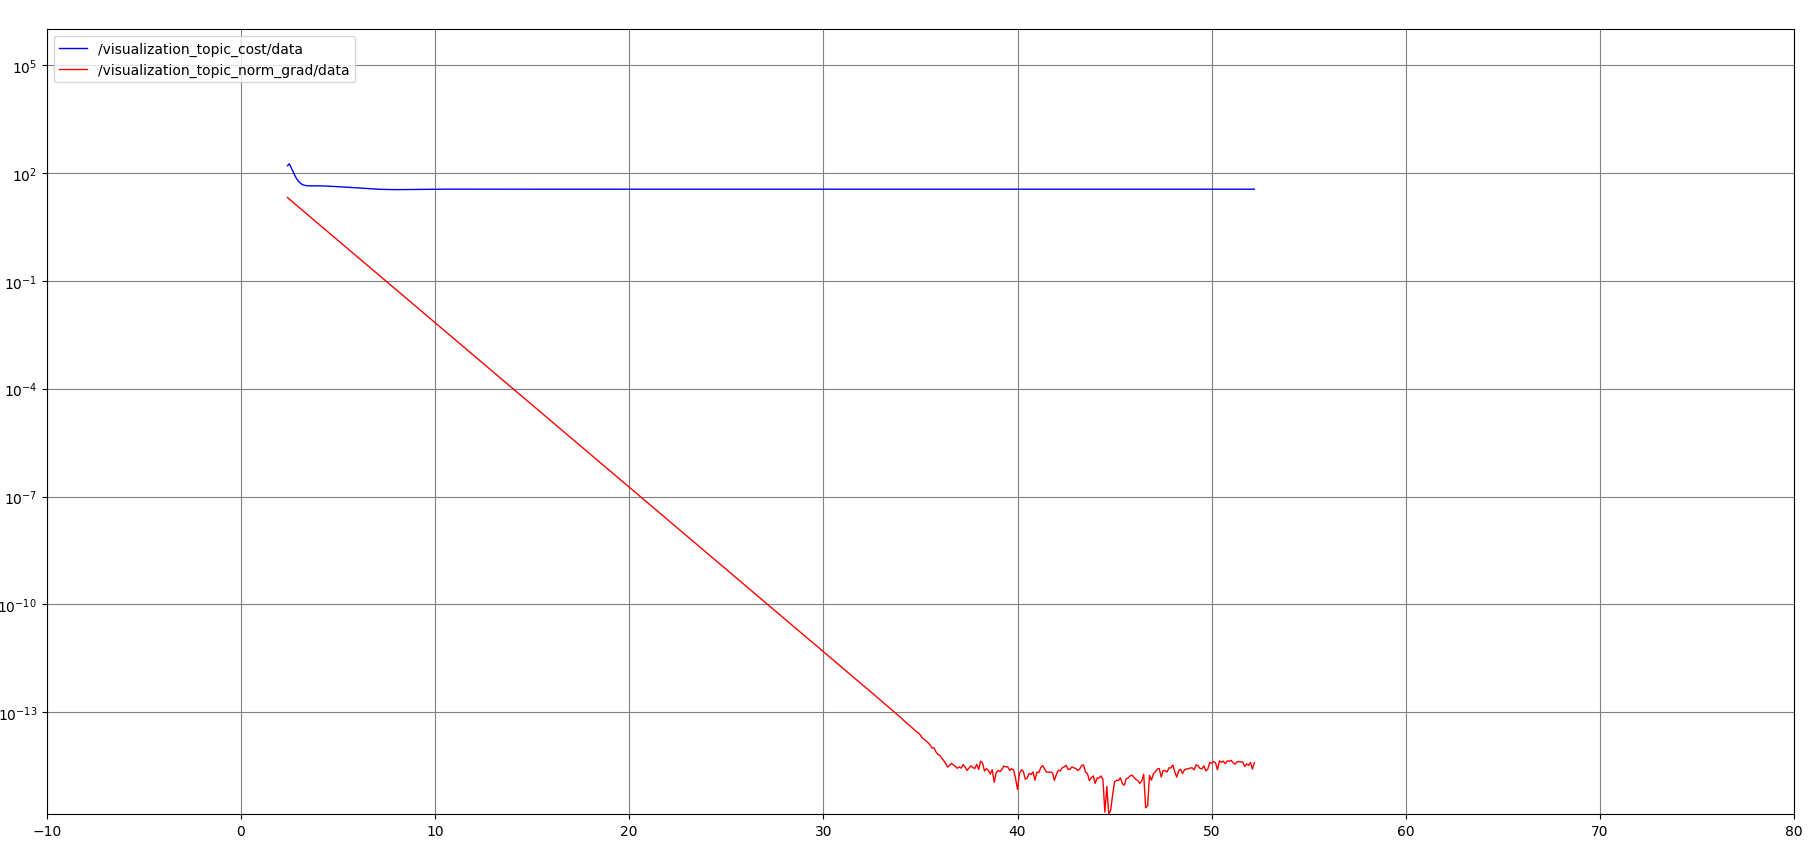
\includegraphics[width=0.7\linewidth]{report/figs/plot_cost_norm.png}
    \caption{Convergence of the gradient norm over time}
    \label{fig:rqt_plot}
\end{figure}

Figure \ref{fig:rviz_result} illustrates the spatial behavior of the agents as visualized in RViz. In addition, Figure \ref{fig:rqt_plot} shows the convergence of the distributed optimization algorithm. The norm of the gradient progressively decreases to zero, confirming the linear convergence predicted by Distributed Aggregative Tracking theorem.